\documentclass[
	%parspace, % Térköz bekezdések közé / Add vertical space between paragraphs
	%noindent, % Bekezdésének első sora ne legyen behúzva / No indentation of first lines in each paragraph
	%nohyp, % Szavak sorvégi elválasztásának tiltása / No hypenation of words
	twoside, % Kétoldalas nyomtatás / Double sided format
	final, % Teendők elrejtése / Set final to hide todos
]{elteikthesis}[2019/06/10]

% Dolgozat metaadatai
% Document's metadata
\title{Automatic Spine Vertebrae Segmentation from CT Images } % cím / title
\date{2021} % védés éve / year of defense

% Szerző metaadatai
% Author's metadata
\author{Kumundzhiev Maxim}
\degree{programtervező informatikus MSc}

% Témavezető(k) metaadatai
% Superivsor(s)' metadata
\supervisor{Szűcs Ádám István} % belső témavezető neve / internal supervisor's name
\affiliation{doctoral candidate} % belső témavezető beosztása / internal supervisor's affiliation
%\extsupervisor{Külső Kornél} % külső témavezető neve / external supervisor's name
%\extaffiliation{informatikai igazgató} % külső témavezető beosztása / external supervisor's affiliation

% Egyetem metaadatai
% University's metadata
\university{Eötvös Loránd Tudományegyetem} % egyetem neve / university's name
\faculty{Informatikai Kar} % kar neve / faculty's name
\department{Komputeralgebra Tanszék} % tanszék neve / department's name
\city{Budapest} % város / city
\logo{elte_cimer_szines} % logo

% Irodalomjegyzék hozzáadása
% Add bibliography file
\addbibresource{thesis.bib}

% A dolgozat
% The document
\begin{document}
	
% Nyelv kiválasztása
% Set document language
%\documentlang{magyar}
\documentlang{english}

% Teendők listája (final dokumentumban nincs)
% List of todos (not in the final document)
\listoftodos[\todolabel]

% Dokumentum beállítások
% Some document settings
% Lábjegyzet folytonos számozása fejezetek között
% Contiunous counting of footnotes among chapters
\counterwithout{footnote}{chapter}

% Tartalomjegyzék oldalszámozásának rejtése
% Hide page numbering of ToC
\newcounter{conpageno}
\let\oldtableofcontents\tableofcontents
\renewcommand{\tableofcontents}{
	\pagenumbering{gobble}
	\oldtableofcontents
	\cleardoublepage
	\setcounter{conpageno}{\value{page}}
	\pagenumbering{arabic}
	\setcounter{page}{\value{conpageno}}
}


% Címlap (kötelező)
% Title page (mandatory)
\maketitle
\topicdeclaration

% Tartalomjegyzék (kötelező)
% Table of contents (mandatory)
\tableofcontents
\cleardoublepage

% Tartalom
% Main content
\chapter{Introduction}
\label{ch:introduction}

Automatic spine vertebrae segmentation 
- The problem definition
- The problem short explanation



\cleardoublepage

\chapter{Medical Imaging}
\label{ch:rworks}

The imaging modalities used in biology and medicine are based on a variety of energy sources, including light, electrons, lasers, X-rays, radionuclides, ultrasound and nuclear magnetic resonance. The images produced span orders of magnitude in scale, ranging from molecules and cells to organ systems and the full body. !!! This is copied from https://link.springer.com/chapter/10.1007/978-3-662-00807-2_109 !!!
The advantages and limitations of each imaging modality are primarily governed by the basic physical and biological principles which influence the way each energy form interacts with tissues, and by the specific engineering implementation for a particular medical or biological application.

\section{Modalities}
Each modality results from a different phenomenon of physics offers doctors (radiologists) an alternative view of the patient. Moreover each modality has it's risks, costs and benefits. All these factors have to be taken into account when choosing type of modality to be issued.

\subsection{X-Ray (X-RAY)}
In 1895, Wilhelm Roentgen explored rays which could pass through wood and human tissues. He called them "x-rays" where "x" was considered as a place-holder for the unknown.

X-Rays are a form of electromagnetic radiation in the same spectrum as visible light and radio waves. Like light, x-rays can be considered as a energy of an x-ray photon. To make x-rays, it can be fired high-energy electrons into matter. In medical-imaging applications, x-rays are sent into tissue. 

Jointly x-rays interactions with matter it can be considered 3 common cases:
\begin{itemize}
    \item Photoelectric Effect
    \newline This effect is the principal effect that makes x-ray useful.
    \item Compton Interaction
    \newline Because of tissues tend to have little variations, Compton Interaction does not give precise information in terms of what is inside the body. 
    \item Rayleigh (Coherent) Scattering
    \newline Upon interacting with the attenuating medium, the photon does not have enough energy to liberate the electron from its bound state.
\end{itemize}

\subsection{Computed Tomography (CT)}
In simplified terms, the idea of computed tomography is to resolve a single -- or a few slices -- slice of an object using many x-ray projections. As the gantry rotates, the scanner collects a 1D x-ray at each angle.

***The CT scanners which designed for purpose of human diagnostic are generally capable of producing images with voxels, where voxel stand for representing a value on a regular grid in three-dimensional space*** ""This is not correct the CT machine produces projection images which can be reconstructed into a 3D volume, which is a scalar field/set of voxels.""

The CT images which are span of x-rays are a form of ionizing radiation. Ionizing radiation is radiation with high enough energy that electrons can be ejected out of their orbitals, creating ions. These ions in large amounts can cause tissue and DNA damages. By this consideration medicine actively limits the amount of ionizing radiation the patient may potentially get.

\item Contrast Agents
\newline
As one of additional practices approaching CT for retrieving human body information, frequently substances can be introduced to the body to add the contrast, what is named as contrast agents. Often agents may be essentially useful for visualising of observations.          

\item Motion Artifacts
\newline
Usually it takes a few seconds to obtain one bit of CT data. The tidiness of the observations depends on whether the patient moved during the acquisition. If so, the resulting transformation will be inconsistent and the reconstructed image will contain errors. But, if the patient's motions are known, meaning a lot of artifacts can be corrected during the reconstruction. On top of it the few automatic methods can be applied to dare to sharpen the image by guessing the motions.

\subsection{Positron Emission Tomography (PET)}      
Similar to CT, PET approaches with ring of detectors to detect radiation. ***The raw data that comes out of a PET scanner is very similar in nature to the Radon transform in CT.***""This is completely wrong as well, the radiation comes from the body, which is injected a radiopharmacon, e.g.: FDG and it is a totally different data than it is from the CT. CT captures density PET detects counts and Standard Uptake Value (SUV) can be calculated."" ***Beyond, unlike CT scans PET ones take a long time to be acquired,***""CT and PET are super fast 4-5 minutes for acquisition, SPECT can be slow or MRI "" meaning the patient motions can cause the problems. Moreover before issuing the measurements it is injected a small amount of positron-emitting radioisotope into the patient. This radioisotope is bound to a metabolite that is used glucose for instance.        

The list of images modalities and corresponding methods varies a lot strictly depending of the use case.
Below it is denoted few more popular directions:
\begin{itemize}
    \item MEG - Magneto Encephalography
    \item EEG - Electro Encephalography
    \item OCT - Optical Coherence Tomography
    \item SPECT - Single-Photon Emission Computed Tomography
\end{itemize}


\section{Image Segmentation}
%ADD VISUALISATION
In terms of medical imaging, segmentation is the process of classifying pixels into groups which corresponds to the same tissue type. Segmentation has many uses cases like a "measure volume of an organ", "render a 3D view of an organ", "surface-based registration" and many others. Further we will descry types of segmentation. 

\subsection{Thresholding}
%ADD VISUALISATION 
The simplest method for classifying pixels based on solely on their intensity values. In thresholding we choose upper and lower bound and select pixels in predefined range.
The problem within simple thresholding is that it does not take into consideration any spatial information, meaning each pixel is evaluated no matter where it is located.    

\subsection{Region Growing}
Unlike basic thresholding, region growing -- which is iterative method -- starts with the small set of seed pixels and grow out from them.

The method functionality can be easily represented within any basic draw editor. To do that we will draw empty grid rectangle and afterwards select interested regions and apply function named "flat fill" with chosen color. As a result it can be noticed the naive functionality handled the problem of tricking-out the selected regions by chosen color. This is so called region growing thresholding.    

\begin{figure}[h]
    \centering
    \subfloat[\centering Empty grid rectangle]{{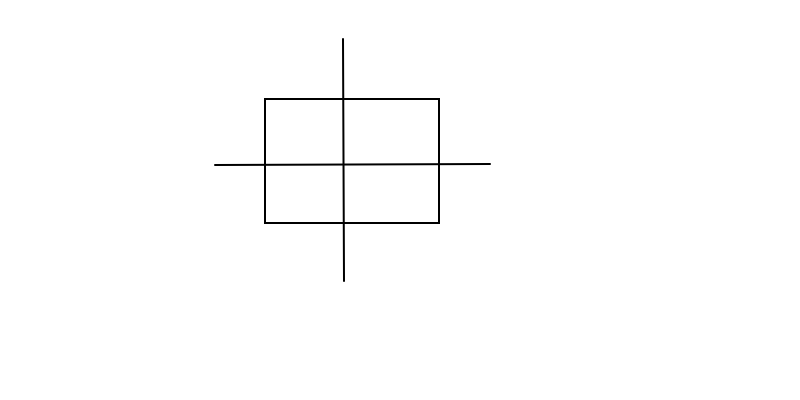
\includegraphics[width=5cm]{images/grow_region_0.png} }}%
    \qquad
    \subfloat[\centering Filled grid rectangle]{{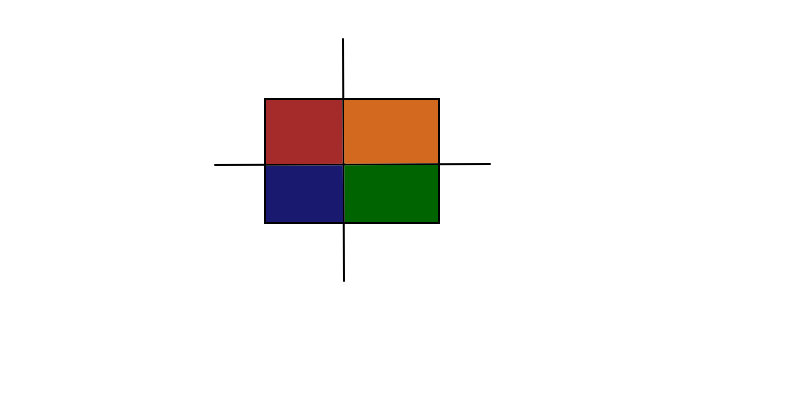
\includegraphics[width=5cm]{images/grow_region_1.png} }}%
    \caption{Region Growing Thresholding}%
    \label{fig:grwoing_region}%
\end{figure}

Now, let us see how it is done from code base perspective.
\begin{lstlisting}
do
  for each pixel in the set
    for each of it's neighbours not in the set
      if the intensity falls between the thresholds
        add it to the set
      endif
    next neighbour
  next pixel
until no pixel were added in the last pass   
\end{lstlisting}

\newcolumntype{C}[1]{>{\centering\let\newline\\\arraybackslash\hspace{0pt}}m{#1}}
\newcolumntype{L}[1]{>{\raggedright\let\newline\\\arraybackslash\hspace{0pt}}m{#1}}

Example: There is set of pixels $4x4$ which should be colored. The cells which denoted by red color is already tricking-out. The task is fill rest with red color based on defined thresholding range.       

\begin{tabular}{C{7cm}  L{7cm}}
    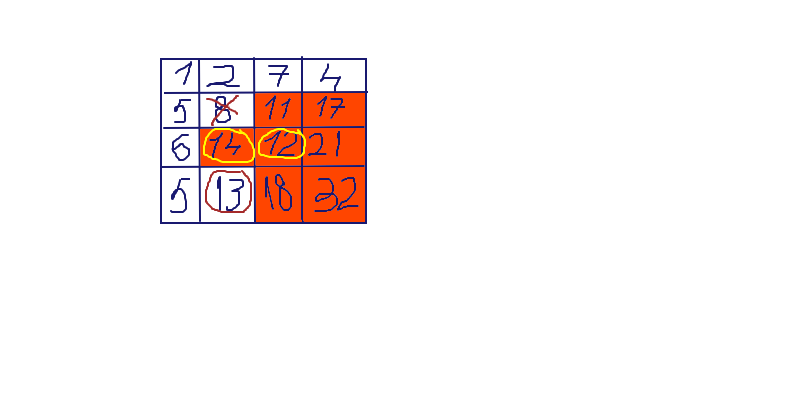
\includegraphics[width=12cm]{images/grow_region_3.png} & Thresholds: include a pixel if $10 \leq intensity \leq 100$ \newline 
    \begin{lstlisting}
    Looking at 14 ...
    up: 8 -> exclude (not in range)
    right: 12 -> skip (already in the set)
    down: 13 -> include as a new entry
    left: 6 -> exclude (not in range)
    \end{lstlisting}
\end{tabular}

Exactly the same way growing region thresholding method may be applied for medical images of different image modalities.
\begin{figure}[h]
    \centering 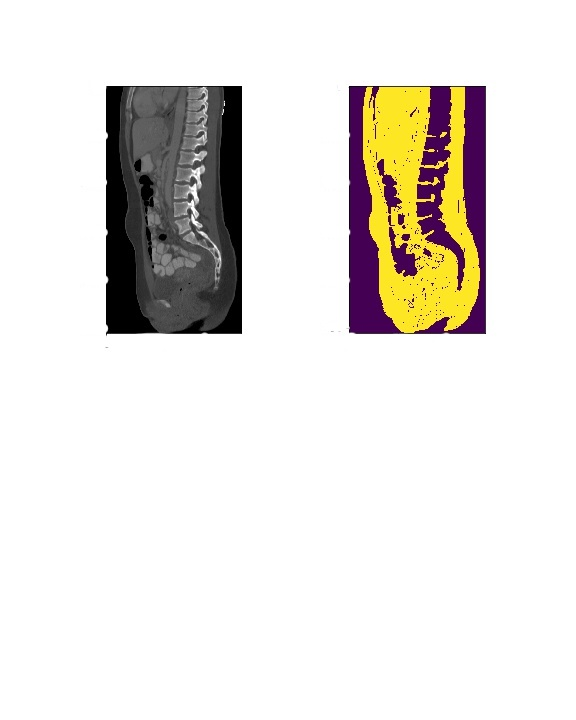
\includegraphics[width=7cm]{images/ct-spine-grow-region-segmented.jpg}
    \vspace*{-30mm} \caption {Original CT spine vs Segmented CT spine with Grow Region thresholding}
\end{figure}    

There is a huge potential room for improvements making the method more sophisticated by coming up with different conditions for inclusion/exclusion of pixels.

\subsubsection{k-Means Clustering}
k-Means algorithm is very simple clustering method whereas usually the data set is represented as the a scatter plot in some feature space.

For instance, a pixel could be represented by 3 dimensional feature space, where feature space is defined by retrieving from the image following pixel-wise features:
\begin{itemize}
    \item Intensity
    \item Gradient magnitude
    \item Laplacian
\end{itemize}

First let us clarify the target results we are looking for by considering the very trivial task.
Assume, there is colorful triangle which should be clustered and represented in some feature space. Afterwards we can clearly see 3 different colors which denotes 3 clusters/groups.
\begin{figure}[h]
    \centering
    \subfloat[\centering colorful triangle]{{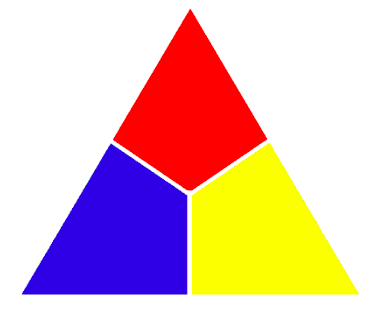
\includegraphics[width=5cm]{images/k_mean_triangle.png} }}%
    \qquad
    \subfloat[\centering feature space representation]{{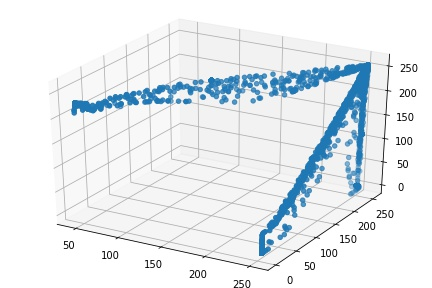
\includegraphics[width=5cm]{images/k_mean_triangle_clustered.jpg} }}%
    \caption{feature space representation after applying k-Means}%
    \label{fig:grwoing_region}%
\end{figure}

As for now, imagine, the user specified k the number of clusters, meaning how many different tissue types are in the image.
Hence, the algorithm may be defined as:
\begin{lstlisting}
1. (randomly) choose k regressors as prototype
2. assign each scatter point ("feature vector") to it's nearest regressor
3. recalculate new prototypes (the mean of it's members)
4. if the prototypes changed significantly -> go to the step 2 
\end{lstlisting}
To demonstrate the method we are going to proceed with the same ct spine scan data which had used for region growing thresholding. As for regressors number (clusters number) we will choose $k=3$.  

\newpage
\begin{figure}[h]
    \centering 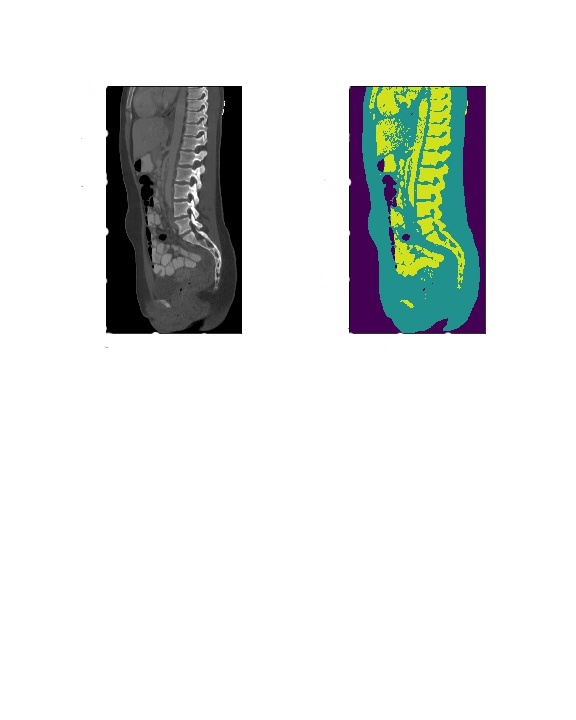
\includegraphics[width=7cm]{images/ct-spine-k-means-segmented.jpg}
    \vspace*{-40mm} \caption {Original CT spine vs Segmented CT spine with k-Means algorithm}
\end{figure}    

As we can see, clustering is a really nice way for image segmentation, because you get to see the joint intensity of scatter plot (feature space) as well as different representations of clusters.  

\subsection{Snakes}
%TBD
Shortly defined, it is active contour which is like a deformable boundary on an image designed to converge to an anatomical boundary of some sort. Deformable boundary is often represented by a number of nodes and vertices.  

\subsection{Level Sets}
%TBD
The level set method is a different way to formulate the active contour idea. %In fact it is the Eulerian formulation and when you explicitly represent the curve it is the Lagrangian formulation


\cleardoublepage


\chapter{Problem Background}
\label{ch:problem_background}

Image segmentation \cite{Shapiro2001} is the process of partitioning a digital image into multiple segments (sets of pixels, also known as image objects). The goal of segmentation is to simplify and/or change the representation of an image into something that is more meaningful and easier to analyze. In mathematical terms, the aim is to find a closed contour $\Gamma$ that partitions a domain $\Omega \in \mathbb{R}$  into subregions $\Omega_i, i = 1, 2, ..., N$.
The very first notation was established by David Mumford $\footnote{ \url{https://en.wikipedia.org/wiki/David_Mumford}}$ in 1989 and obtained name \cite{Kim2020} Mumford-Shah functional.

\section{Mumford-Shah functional}
Mumford-Shah functional considers the piecewise smooth approximation of an input image $z(x)$ by a pair $(\upsilon, \Gamma)$. Assume $\Omega$ be a bounded domain in $\mathbb{R}$ and $z(x)$ be a bounded measurable function defined on $\Omega$. The functional is defined as follows:
\begin{align*}
 E (\upsilon, \Gamma) = \upsilon H^{n-2} (\Gamma) + \mu^2 \int_{\Omega} (\upsilon - z)^2 \partial x + \int_{\frac{\Omega}{\Gamma}} \lvert \nabla \upsilon \rvert^2 \partial x
 \end{align*}

The functional contains a fidelity term on $\upsilon \in \complement^1$ and two regularity terms. One
imposes smoothness on $\upsilon$ and the others imposes regularity on $\Gamma$ in terms of its one dimensional \cite{Buda1992} Hausdorff measure.

Mumford and Shah also introduced the restriction of $E$ to piecewise-constant functions $\upsilon$. In other words $\upsilon = c_k$ on each open set $\Omega_k$, where $c_k$ stands for average value of $z$ in each region $\Omega_k$. The piecewise-constant Mumford-Shah functional is defined as:

\begin{align*}
 E_0 (\upsilon, \Gamma) = \upsilon H^{n-1} (\Gamma) \int_{\Omega_k} (\upsilon - c_k)^2 \partial x
\end{align*}

It can be proved that $E_0$ is the natural limit functional of $E$ as $\mu \to 0$. This is linked, in the discrete setting, to the \cite{Wu1982} Potts Model which has been widely studied. The above functional is the basis for a significant amount of important work in field of image segmentation.
\cleardoublepage




% Irodalomjegyzék (kötelező)
% Bibliography (mandatory)
\addcontentsline{toc}{chapter}{\biblabel}
\printbibliography[title=\biblabel]
\cleardoublepage

% Ábrajegyzék (opcionális) - 3-5 ábra fölött érdemes
% List of figures (optional) - useful over 3-5 figures
%\addcontentsline{toc}{chapter}{\lstfigurelabel}
%\listoffigures
%\cleardoublepage

% Táblázatjegyzék (opcionális) - 3-5 táblázat fölött érdemes
% List of tables (optional) - useful over 3-5 tables
%\addcontentsline{toc}{chapter}{\lsttablelabel}
%\listoftables
%\cleardoublepage

% Forráskódjegyzék (opcionális) - 3-5 kódpélda fölött érdemes
% List of codes (optional) - useful over 3-5 code samples
%\addcontentsline{toc}{chapter}{\lstcodelabel}
%\lstlistoflistings
%\cleardoublepage

% Jelölésjegyzék (opcionális)
% List of symbols (optional)
%\printnomenclature

\end{document}
